\documentclass[12pt]{article}
% include the pckage of the color%
\usepackage[usenames, dvipsnames]{color}
\usepackage[english]{babel}
\usepackage[utf8x]{inputenc}
\usepackage{amsmath}
\usepackage{graphicx}
\usepackage{array}

%define your own color %
\definecolor{mygray}{gray}{0.9}



\begin{document}
\listoffigures
	
\title{Chapter 4 : Implementation}
\maketitle
	\section{Introduction}
	
	In this chapter we will focus on the technologies. 
	\section{Java Platform, Enterprise Edition (Java EE)}
		\begin{figure}[h]
		\centering
		
\includegraphics[width=0.4\textwidth]{JAVAEE_logo.png}
		\caption{Java Enterprise Edition logo}
		
	    \end{figure}

\subsection{Introduction}
\textbf{Java EE} is the Java platform edition for Enterprise Software, extending \textbf{Java SE} with APIs for enterprise features such as distributed computing and web services. Java EE applications are run on an application server, which handle transactions, security, scalability, concurrency and management of the components it is deploying.
\\
\\
The platform was known as \textit{Java 2 Platform, Enterprise Edition or J2EE} from version 1.2 (December 12, 1999), until the name was changed to \textit{Java Platform, Enterprise Edition} or \textit{Java EE} in version 1.5. The current version is called \textit{Java EE 8}.
\subsection{Features}
The main advantages of using Java EE are :
\begin{itemize}
	\item \textbf{Portability}
	\item \textbf{Independence}
	\item \textbf{Security}
	\item \textbf{The multitude of libraries it offers}
\end{itemize}
The Java EE platform is based on specifications, which means projects are portable on any compliant application server (GlassFish, JBoss...) to these specifications. This implementation is free and allows you to benefit from the entire API without any investment. The Java EE platform is the richest of Java platforms and provides a standard environment for multi-tenant business application development and execution. 
\\
\\
The JEE platform provides the following :
\begin{itemize}
	\item Complete Web services support. The JEE platform provides a framework for developing and deploying web services on the Java platform. 
	\item The Java API for XML-based RPC (JAX-RPC) enables Java technology developers to develop SOAP based interoperable and portable web services.
	\item Developers use the standard JAX-RPC programming model to develop SOAP based web service clients and endpoints.
	\item A web service endpoint is described using a Web Services Description Language (WSDL) document.
	\item JAX-RPC enables JAX-RPC clients to invoke web services developed across heterogeneous platforms. In a similar manner, JAX-RPC web service endpoints can be invoked by heterogeneous clients
\end{itemize}

\subsection{Motivation}
According to a trused source "TIOBE index", Java is the most popular language ever.
The TIOBE Programming Community index [1] is an indicator of the popularity of programming languages. The index is updated once a month. The ratings are based on the number of skilled engineers world-wide, courses and third party vendors. Popular search engines such as Google, Bing, Yahoo!, Wikipedia, Amazon, YouTube and Baidu are used to calculate the ratings.
	\begin{figure}[h]
	\centering
	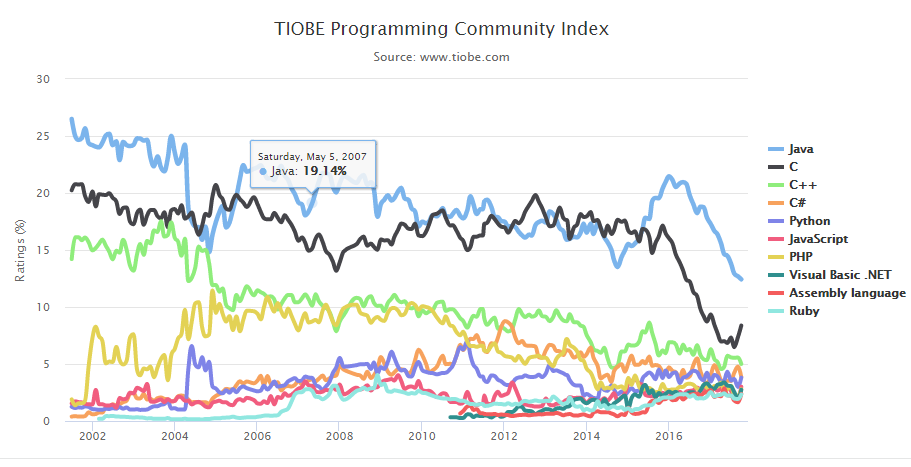
\includegraphics[width=1.0\textwidth]{Java_statics.png}
	\caption{java statics}
    \end{figure}
	\begin{figure}[h]
	\centering
	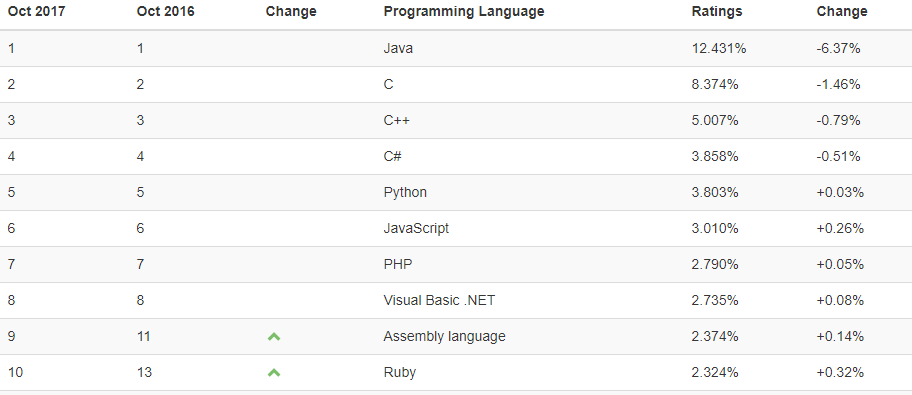
\includegraphics[width=1.0\textwidth]{Java_rank.png}
	\caption{java rank}
    \end{figure}
 As the above statics shows, JAVA is the most used language in the industry, today java it is not an option, it is requirement for almost all the IT Job Apply. \\Other Major key that push us to use java as language of programming in our project (MassTerInsight) [2] is that the core business of MassTer software [3] is developed using java, as results it is easy to integrate in our project without any midelware or such web services.    
\vspace{66mm}
	\section{Angular JS}
		\begin{figure}[h]
		\centering
		
\includegraphics[width=0.3\textwidth]{AngularJS_logo.png}
		\caption{AngularJS logo}
	\end{figure}
		\subsection{Introduction}
	AngularJS is a structural framework for dynamic web apps. It lets you use HTML as your template language and lets you extend HTML's syntax to express your application's components clearly and succinctly. AngularJS's data binding and dependency injection eliminate much of the code you would otherwise have to write.  And it all happens within the browser, making it an ideal partner with any server technology.
	\\
	\\
	AngularJS is what HTML would have been, had it been designed for applications. HTML is a great declarative language for static documents. It does not contain much in the way of creating applications, and as a result building web applications is an exercise \textit{in what do I have to do to trick the browser into doing what I want?}
	\\
	\\
	The impedance mismatch between dynamic applications and static documents is often solved with:
	\begin{itemize}
		
		\item \textbf{a library} - a collection of functions which are useful when writing web apps. Your code is in charge and it calls into the library when it sees fit. E.g., \colorbox{mygray}{jQuery}.
		\item \textbf{frameworks} - a particular implementation of a web application, where your code fills in the details. The framework is in charge and it calls into your code when it needs something app specific. E.g., \colorbox{mygray}{durandal}, \colorbox{mygray}{ember}, etc.
	\end{itemize}
	AngularJS takes another approach. It attempts to minimize the impedance mismatch between document centric HTML and what an application needs by creating new HTML constructs. AngularJS teaches the browser new syntax through a construct we call directives. Examples include:
	\begin{itemize}
		\item Data binding, as in \colorbox{mygray}{\{\{\}\}}
		\item DOM control structures for repeating, showing and hiding DOM fragments.
		\item Support for forms and form validation.
		\item Attaching new behavior to DOM elements, such as DOM event handling.
		\item Grouping of HTML into reusable components.	
	\end{itemize}
	\subsection{Features}
	\begin{itemize}
		\item AngularJS is a powerful JavaScript based development framework to create RICH Internet Application(RIA).
		\item  AngularJS provides developers options to write client side application (using JavaScript) in a clean MVC(Model View Controller) way.
		\item  Application written in AngularJS is cross-browser compliant. AngularJS automatically handles JavaScript code suitable for each browser.
		\item AngularJS is open source, completely free, and used by thousands of developers around the world. It is licensed under the Apache License version 2.0.
	\end{itemize}
		Overall, AngularJS is a framework to build large scale and high performance web application while keeping them as easy-to-maintain.
		\\
		\\
		We present in this table the directives used in our project.
		\\
		\\
		\begin{tabular}{|l|c|r|}
			\hline
			\textbf{Directive} & \textbf{description }\\
			\hline
			ng-app & .. \\
			ng-model & ..  \\
			ng-switch & .. \\
			ng-switch-when & ..  \\	
			\hline
		\end{tabular} 
	\subsection{Motivation}
	Before I started to choose any javascript frameworks, I made a research on who are the most used and best javascript framework in the world ?
	\\
	Almost all the articales That I read shows that the most popular frameworks are \colorbox{mygray}{angularjs}, \colorbox{mygray}{ember JS}, \colorbox{mygray}{react JS} and \colorbox{mygray}{backbone JS}, AngularJS is the most used framework amongst these framworks and this is my first motivation.\\
	Second, The community behind angularjs is the community google, recent updates, large used by the developers as resultats resolved the bugs, also impovements.\\
	The industry in our country and all the world, the jobs requirements skills tend to require more and more the framework angularjs base on recent research on google Trends(see the figure N°) .
	 	\begin{figure}[h]
	 	\centering
	 	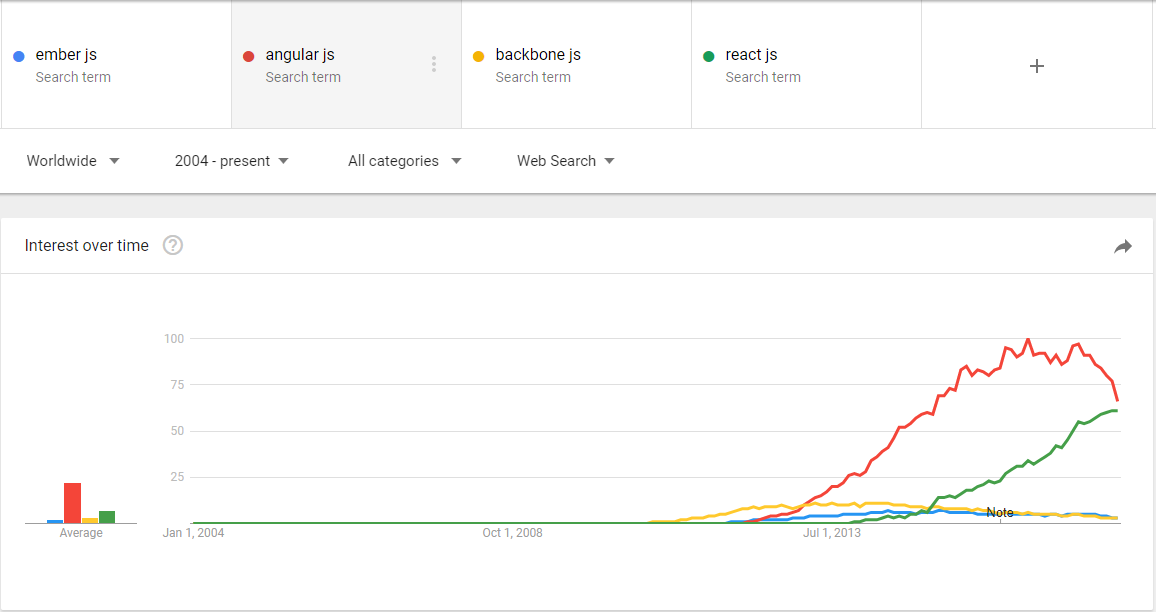
\includegraphics[width=1.0\textwidth]{AngularJS_statics_google_trends.png}
	 	\caption{AngularJS on google trends}
	 \end{figure}
	 
	
	\section{Bootstrap}
	\begin{figure}[h]
		\centering
		
\includegraphics[width=0.20\textwidth]{Boostrap_logo.png}
		\caption{Bootstrap logo}
	\end{figure}
	\subsection{Introduction}
	\textbf{Bootstrap} is a free and open-source front-end web framework for designing websites and web applications. It contains HTML- and CSS-based design templates for typography, forms, buttons, navigation and other interface components, as well as optional JavaScript plugins. Unlike many web frameworks, it concerns itself with front-end development only.
	\\
	\\
	Bootstrap was developed by Mark Otto and Jacob Thornton at Twitter, and released as an open source product in August 2011 on GitHub.\\
	\textbf{In June 2014 Bootstrap was the No.1 project on GitHub!}
	\subsection{Features}
	\textbf{Bootstrap 3} supports the latest versions of the \textbf{Google Chrome}, \textbf{Firefox}, \textbf{Internet Explorer}, \textbf{Opera}, and \textbf{Safari} (except on Windows). It additionally supports back to IE8 and the latest Firefox Extended Support Release (ESR).
	\\
	Since \textbf{2.0}, \textbf{Bootstrap} supports \textbf{responsive web design}. This means the layout of web pages adjusts dynamically, taking into account the characteristics of the device used (desktop, tablet, mobile phone).
	\\
	Starting with \textbf{version 3.0}, Bootstrap adopted a mobile-first design philosophy, emphasizing responsive design by default.
	\\
	The \textbf{version 4.0} alpha release added \textbf{Sass} and \textbf{flexbox} support
	\subsection{Motivation}
	All the researchs shows that Bootstrap The most popular HTML, CSS, and JavaScript framework for developing responsive, mobile first projects on the web.
	\\
	According to github, Bootstrap is the second starred repository, with \textbf{115k stars}.
		\begin{figure}[h]
		\centering
		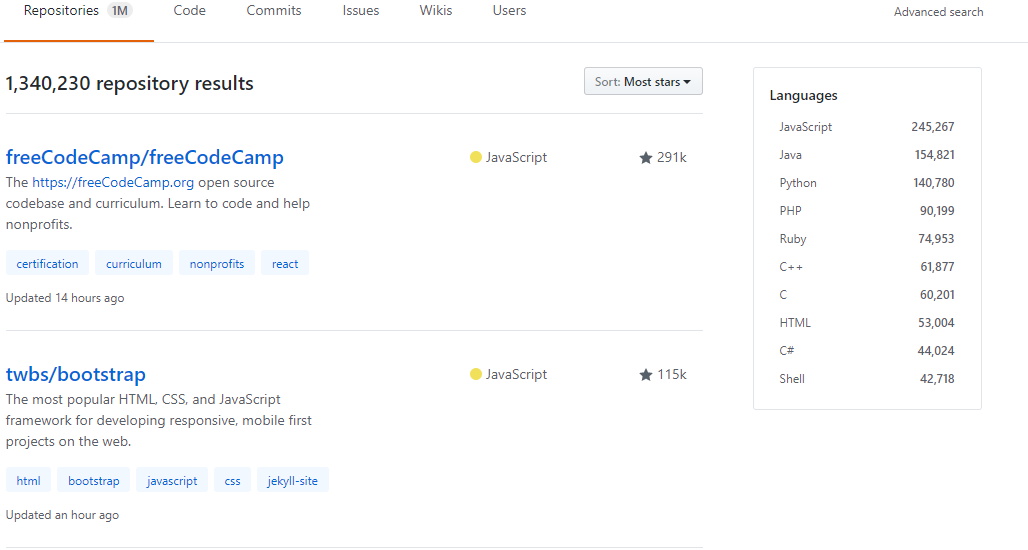
\includegraphics[width=1\textwidth]{Boostrap_statics_github.png}
		\caption{Bootstrap second starred on github}
	\end{figure}

\vspace{66mm}

According to a researchs in the net, all the high-tech blogs encourage developers to use bootstrap.
\\
\\
 I used a tool offred by google named \textbf{google trends} to make a compraison between a subjects in term of most researched.
 \\
 After this compraison in google trends, Bootstrap also is the most googled css framework on the web , compared to the others css frameworks Eg. \textbf{Material UI} which was considered as the most popular css framework after Bootstrap.

\begin{figure}[h]
	\centering
	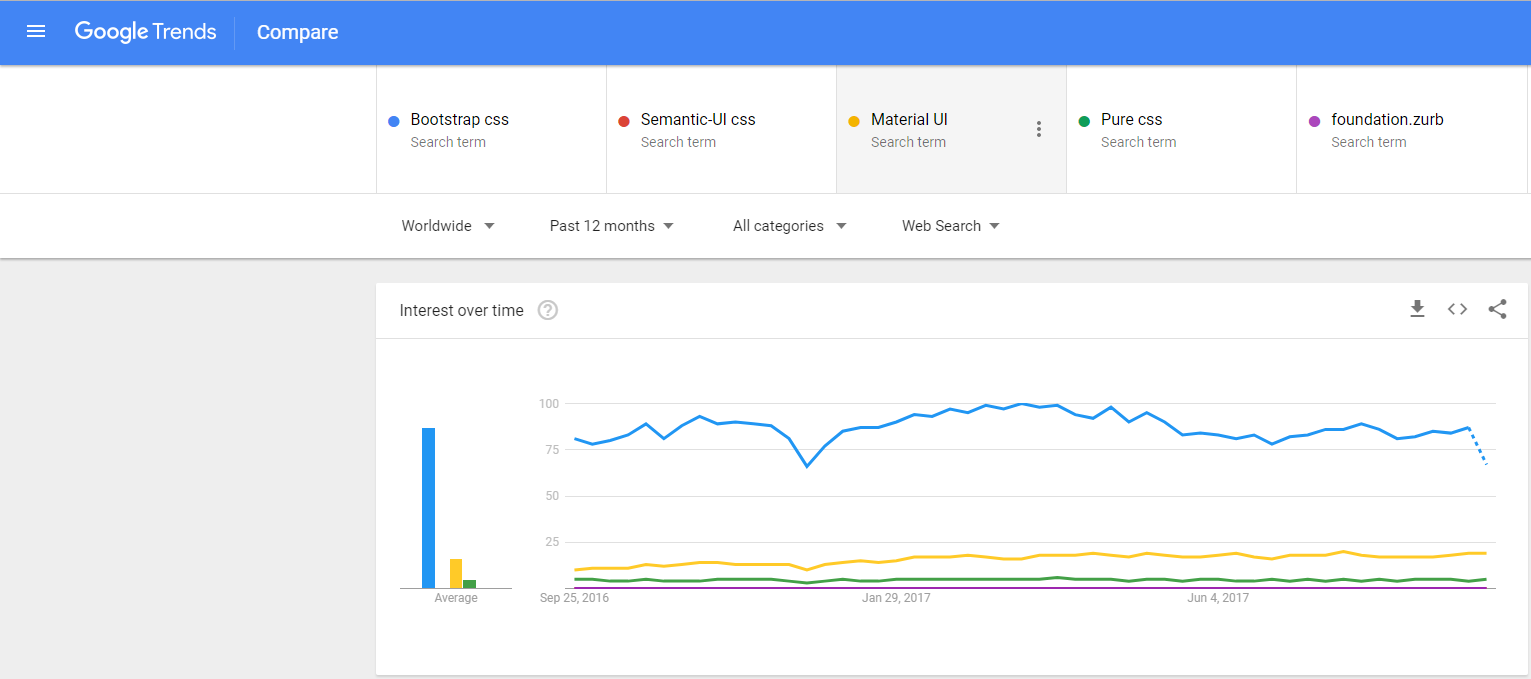
\includegraphics[width=1\textwidth]{Boostrap_statics_google_trends.png}
	\caption{Bootstrap on google trends}
\end{figure}
\vspace{66mm}
\section{Spring mvc framework}
\begin{figure}[h]
	\centering
	
\includegraphics[width=0.4\textwidth]{Spring_logo.png}
	\caption{Spring logo}
\end{figure}
\subsection{Introduction}
The Spring Web model-view-controller (MVC) framework is designed around a \colorbox{mygray}{DispatcherServlet} that dispatches requests to handlers, with configurable handler mappings, view resolution, locale, time zone and theme resolution as well as support for uploading files. The default handler is based on the \colorbox{mygray}{@Controller} and \colorbox{mygray}{@RequestMapping} annotations, offering a wide range of flexible handling methods. With the introduction of Spring 3.0, the \colorbox{mygray}{@Controller} mechanism also allows you to create RESTful Web sites and applications, through the \colorbox{mygray}{@PathVariable} annotation and other features.
 \\
\\
Spring’s web MVC framework is, like many other web MVC frameworks, request-driven, designed around a central Servlet that dispatches requests to controllers and offers other functionality that facilitates the development of web applications. Spring’s \colorbox{mygray}{DispatcherServlet} however, does more than just that. It is completely integrated with the Spring IoC container and as such allows you to use every other feature that Spring has.
\\
\\
The request processing workflow of the Spring Web MVC \colorbox{mygray}{DispatcherServlet} is illustrated in the following diagram. The pattern-savvy reader will recognize that the \colorbox{mygray}{DispatcherServlet} is an expression of the ``Front Controlle'' design pattern (this is a pattern that Spring Web MVC shares with many other leading web frameworks).
\begin{figure}[h]
	\centering
	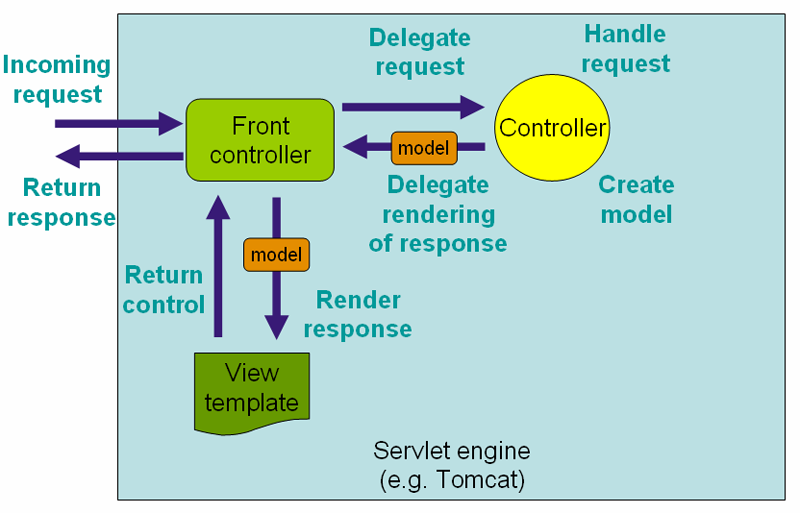
\includegraphics[width=1.1\textwidth]{workflow_spring_mvc.png}
	\caption{The request processing workflow in Spring Web MVC}
\end{figure}
\vspace{66mm}
\subsection{Features}
\begin{itemize}
	\item Since Spring MVC framework is designed like any other Spring module, developer need not spend any extra time to learn it.
	\item Since all the layers are independent of each others, unit testing can be easier.
	\item Spring framework doesn’t force you to follow any pattern, or implementations to write your business logic. So it gives developer flexibility to implement or integrate any other design pattern to suffice his needs.
	\item Spring provides good separation flexibility between Controller, Service and Data access layers.
	\item Spring provides you with a tag library that is simple and yet very powerful.
	\item View side you can integrate with any UI framework like JSF, Velocity, Freemarker etc.
	\item Supports Annotation based programming along with XML, which makes development faster and cleaner.
	
	We present in this table the annotations used in our project :
	\\
	\\
	\begin{tabular}{|l|c|r|}
		\hline
		\textbf{Annotation} & \textbf{description }\\
		\hline
		Controller & .. \\
		ModelView & ..  \\
		RequestBody & .. \\
		RespeseBody & ..  \\	
	    @RequestMapping & .. \\
		\hline
	\end{tabular}
	

\end{itemize} 
\subsection{Motivation}
According to trusted sources like google engine, yahoo, Linkedin and satckoverflow: sping mvc, struts And JSF are the most JEE frameworks searched and posted by the developers, Let's take a look on google trends !!.\\
\begin{figure}[h]
	\centering
	\includegraphics[width=1.0\textwidth]{SpringMVC_statics_google_trends.png}
	\caption{Spring framework on google trends}
\end{figure}
\\
As you can see the curve of spring mvc is very high, wich means that spring is the most used among others frameworks, another key is That spring is the most framework recommend on job application.
\\
\\
The community behind spring is very active, recent updates, less bugs, imrpovement and high performance.
\section{Pivotal tc Server}
\section{spring tools suits}
\section{Apache Maven}
\begin{figure}[h]
	\centering
	
\includegraphics[width=0.5\textwidth]{Maven_logo.png}
	\caption{Apache Maven logo}
\end{figure}
\subsection{Introduction}

Apache Maven is a software project management and comprehension tool.\\Based on the concept of a project object model (POM), Maven can manage a project's build, reporting and documentation from a central piece of information.\\

\subsection{Features}
Maven provides the following benefits :
\begin{itemize}
	\item Able to easily work with multiple projects at the same time.
	\item A large and growing repository of libraries and metadata to use out of the box, and arrangements in place with the largest Open Source projects for real-time availability of their latest releases
	\item Model based builds: Maven is able to build any number of projects into predefined output types such as a JAR, WAR, or distribution based on metadata about the project, without the need to do any scripting in most cases.
	\item Dependency management: Maven encourages the use of a central repository of JARs and other dependencies.
	\item Maven comes with a mechanism that your project's clients can use to download any JARs required for building your project from a central JAR repository much like Perl's CPAN.
	\item This allows users of Maven to reuse JARs across projects and encourages communication between projects to ensure that backward compatibility issues are dealt with.
\end{itemize}
\section{HTML5}
\begin{figure}[h]
	\centering
	
\includegraphics[width=0.3\textwidth]{HTML5_logo.png}
	\caption{HTML5 logo}
\end{figure}
\subsection{Introduction}
HTML5 is the next major revision of the HTML standard superseding HTML 4.01, XHTML 1.0, and XHTML 1.1. HTML5 is a standard for structuring and presenting content on the World Wide Web.
\subsection{Features}
HTML5 introduces a number of new elements and attributes that helps in building a modern website. Following are great features introduced in HTML5.
\begin{itemize}
	\item \textbf{New Semantic Elements} − These are like <header>, <footer>, <aside> and <section>.
	\item \textbf{Forms 2.0} − Improvements to HTML web forms where new attributes have been introduced for <input> tag.
	\item \textbf{Persistent Local Storage} − To achieve without resorting to third-party plugins.
	\item \textbf{WebSocket} − A a next-generation bidirectional communication technology for web applications.
	\item \textbf{Server-Sent Events} − HTML5 introduces events which flow from web server to the web browsers and they are called Server-Sent Events (SSE).
	\item \textbf{Canvas} − This supports a two-dimensional drawing surface that you can program with JavaScript.
	\item \textbf{Audio \& Video} − You can embed audio or video on your web pages without resorting to third-party plugins.
	\item \textbf{Geolocation} − Now visitors can choose to share their physical location with your web application.
	\item \textbf{Microdata} − This lets you create your own vocabularies beyond HTML5 and extend your web pages with custom semantics.
	\item \textbf{Drag and drop} − Drag and drop the items from one location to another location on a the same webpage.
\end{itemize}	
\end{document}